\section{How BARL Helps Generalization: A Didactic Example}\label{sec_example}
\begin{wrapfigure}{r}{0.24\textwidth}
        \vspace{-0.35cm}
    \begin{minipage}[t]{0.24\textwidth}
        \centering
        \begin{minipage}[t]{\linewidth}
            \centering
            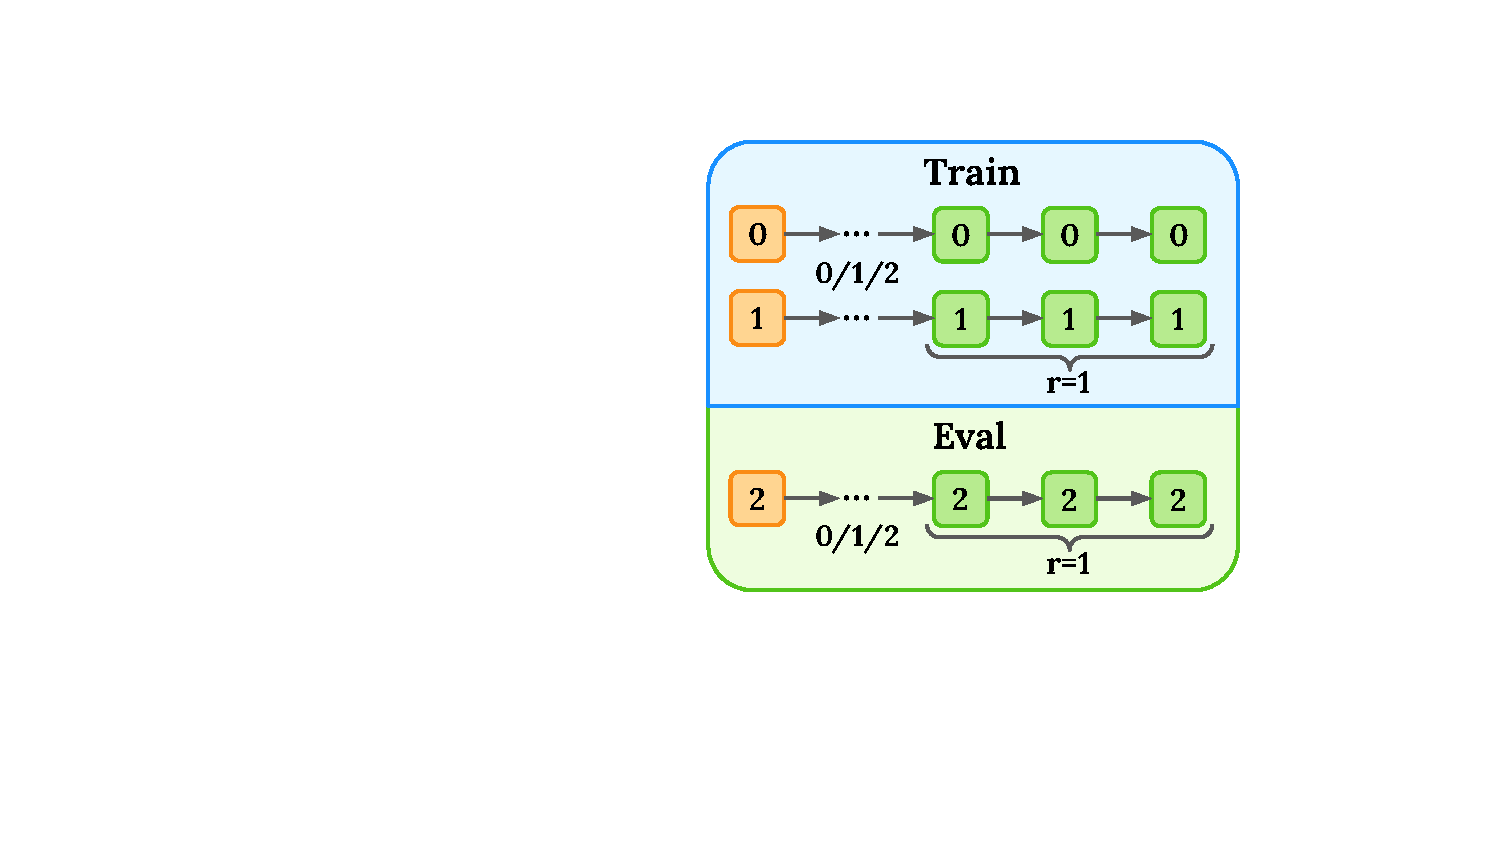
\includegraphics[width=\linewidth]{figs/bamdp_illu_new.pdf}
        \end{minipage}
        \vspace{-0.62cm}
        \setlength{\belowcaptionskip}{-15pt}
        \caption{Setup: repeating the prompt token (orange) three times receives a $1$ reward.}
        \label{fig_illu}
    \end{minipage}
\end{wrapfigure}
Now we present a didactic example to show how BARL facilitates eest-time generalization. Consider the action space $\mathcal{A}$ that consists of three tokens, $\{0, 1, 2\}$, with one token generated at each timestep. The objective is to repeat the prompt token three times consecutively within $29$ timesteps ($3^3+2$ is the minimal length to include all unique triplets). The prompt token is $0$ or $1$ during training, which does not have coverage for $2$. After training, the policy is deployed, where we consider the prompt token of $2$ as the evaluation task. Episodes terminate when receiving a $1$ reward. This setup is illustrated in Figure \ref{fig_illu}.

This setup mirrors LLM reasoning, where the goal is to not only learn specific strategies (here, generating particular triplets), but also general problem-solving abilities, such as when and how to switch to new strategies. These capabilities are essential for handling distribution shifts between training and eval, a common challenge when developing LLMs.

We use a $2$-head transformer encoder followed by a linear layer as the policy and train it using the policy gradient from conventional RL and from BARL \eqref{eq_bayes_gradient}. For RL, the state-action value $Q^{\pi_\theta}$ in the policy gradient is $1$ only when $s_{0:T-1}$ contains the rewarding triplet $\argmax_{\text{tri}}r(\text{tri})$ of the ground-truth MDP, such as $000$ or $111$ during training. For BARL, we set $\beta=\infty$ so that $\prod_{t'=0}^{t-1}\exp(-\beta|r_{t'} - r_{\mathcal{M}_i}(s_{t'}, a_{t'})|) = \mathbbm{1}(\argmax_{\text{tri}}r_{\mathcal{M}_i}(\text{tri})\notin s_{0:t})$, i.e., the product is $0$ when the rewarding triplet of $\mathcal{M}_i$ already appears in $s_{0:t}$ (since $r_{t'}=0$ for unterminated sequences) and $1$ otherwise. For the policy's state-conditional belief $p(\mathcal{M}| s_{0:t})$, sampling from it is equivalent to sampling $a_{t}\sim\pi_\theta(\cdot|s_t)$, with the associated $\mathcal{M}$ satisfying $\argmax_{\text{tri}}r_{\mathcal{M}}(\text{tri}) = s_{t-1:t+1}$. Therefore,
\$
\vspace{0.2cm}
\EE_{\mathcal{M}}\bigl[Q^{\pi_\theta}_\mathcal{M}(s_t, a_t)\bigr] = \EE_{\mathcal{M}\sim p(\mathcal{M}|s_{0:t})}\bigl[Q^{\pi_\theta}_\mathcal{M}(s_t, a_t)\mathbbm{1}(\argmax_{\text{tri}}r_{\mathcal{M}}(\text{tri})\notin s_{0:t})\bigr] = \EE_\pi\bigl[\mathbbm{1}(s_{t-1:t+1}\notin s_{0:t})\bigr].
\$
The above formulation incentivizes the policy to eliminate hypotheses and switch to new strategies (i.e., new triplets) when the current strategy has been invalidated by earlier attempts up to step $t$, which is illustrated in Figure \ref{fig_example_how}. This form of adaptive exploration provides a minimalist instantiation of BARL in synthetic settings. The difference between the above equation and \eqref{eq_adv_algo} arises because the agent here is aware of the zero reward associated with unfinished episodes.

\begin{figure*}[htbp]
    \centering
    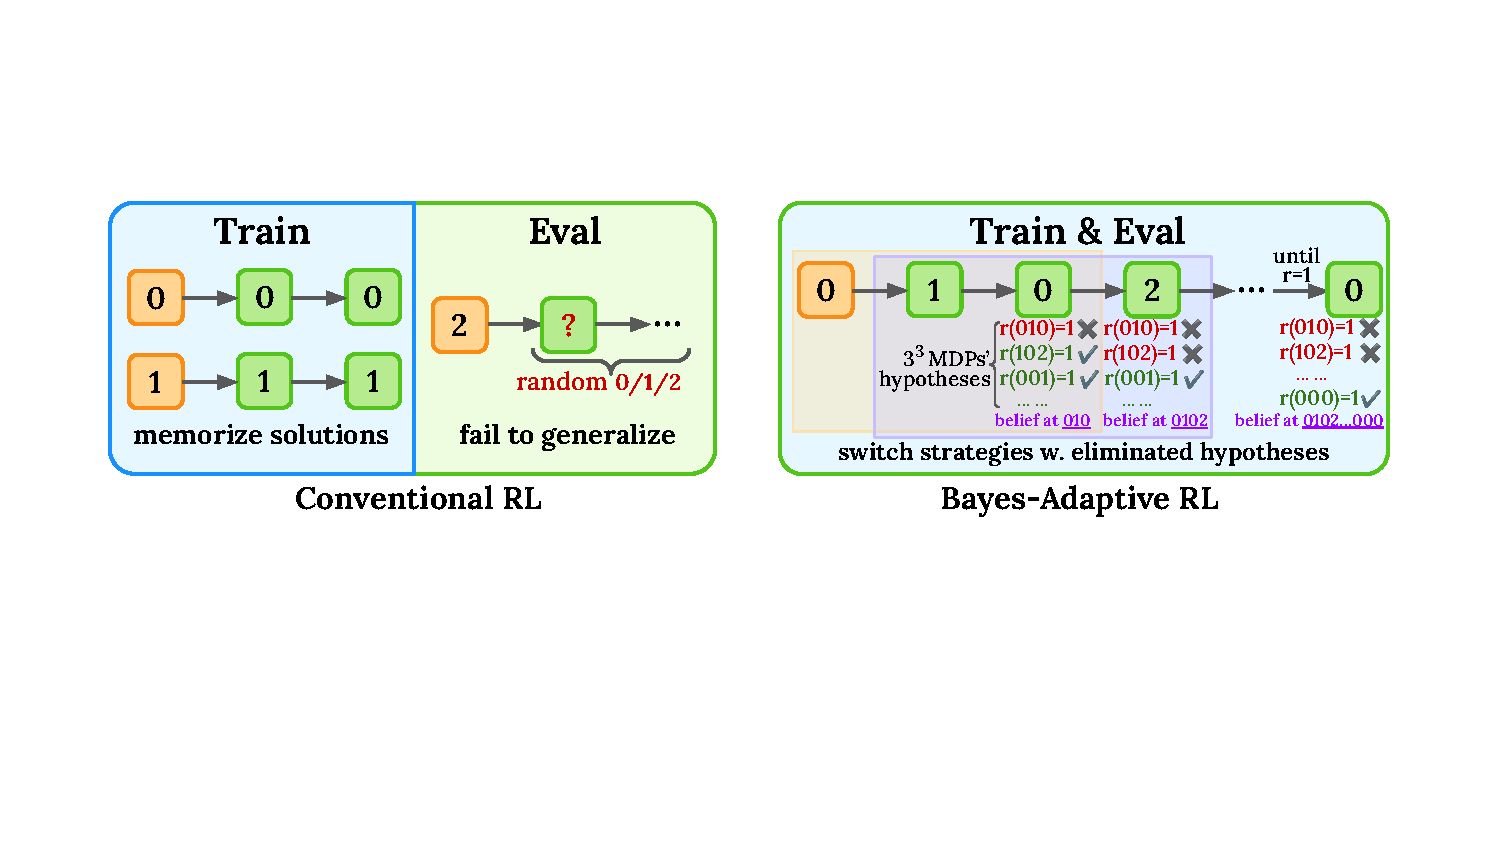
\includegraphics[width=0.75\linewidth]{figs/example_how_new.pdf}
\vspace{-0.1cm}
  \caption{Illustration of the difference between Markovian RL and BARL in this didactic example.}
    \label{fig_example_how}
\end{figure*}

We report the results in Figure \ref{fig_example_results}, where accuracies are averaged over $50$ completions and the shadow regions are the standard deviation across $3$ independent model training runs. The results show that RL quickly finds and memorizes the training solutions but fails to generalize when deployed to the evaluation tasks. In contrast, Bayes-Adaptive RL significantly increases the evaluation accuracies. Furthermore, the accuracy and convergence rate improve when given prior knowledge that rewarding triplets are repeated patterns, i.e., $|\mathcal{M}|=3$ with $r_{\mathcal{M}_1}(000) = r_{\mathcal{M}_2}(111) = r_{\mathcal{M}_3}(222) = 1$. This highlights the advantage of more informative candidate sets, underscoring the importance of balancing \textit{diversity} and \textit{plausibility} of the candidates. Specifically, they should be diverse enough to capture deployment-time uncertainty, yet constrained to only the most plausible candidates to shrink the hypothesis space.
\begin{figure}[h]
    \centering
    \begin{minipage}[b]{0.32\linewidth}
        \centering
        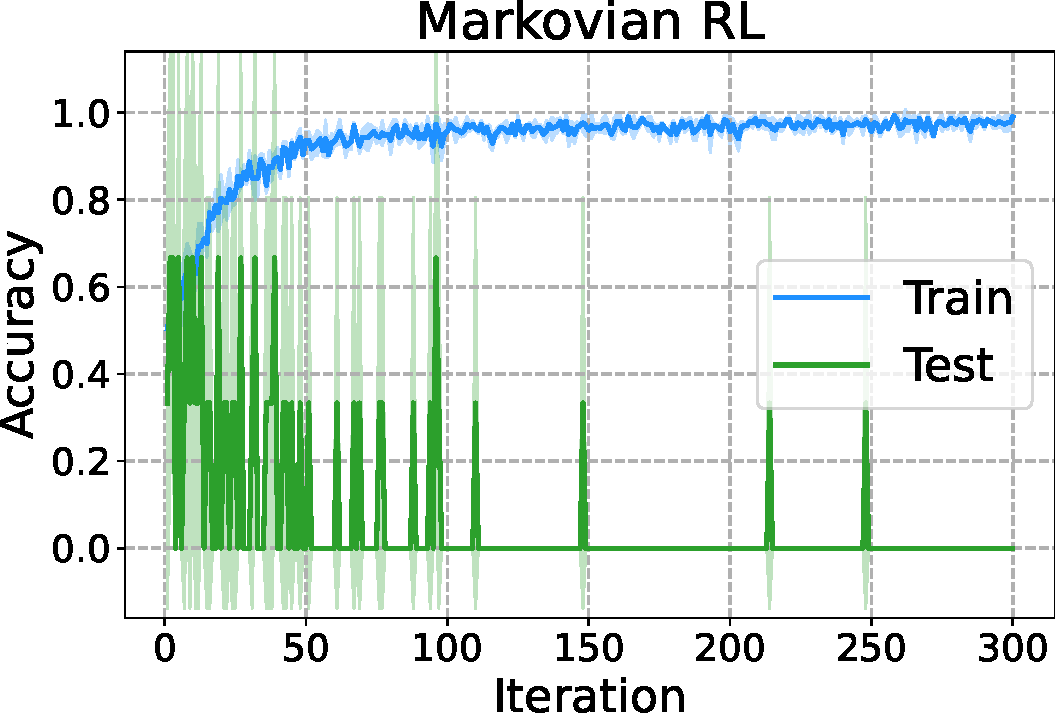
\includegraphics[width=0.96\linewidth]{figs/markovian_example.pdf}
    \end{minipage}
    \begin{minipage}[b]{0.32\linewidth}
        \centering
        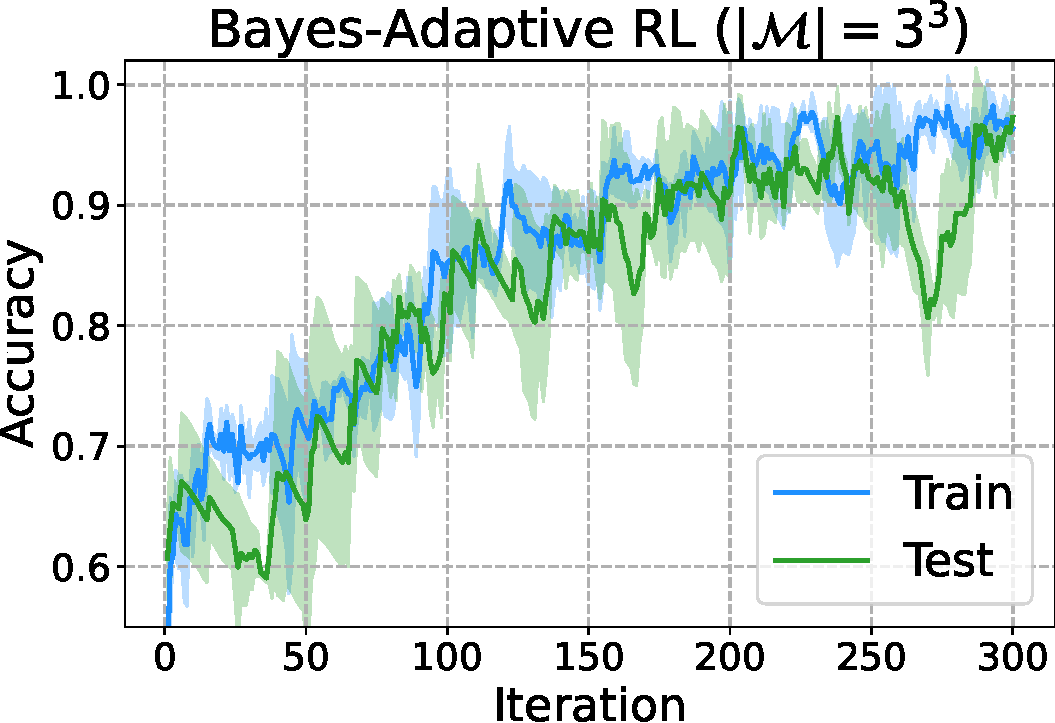
\includegraphics[width=0.96\linewidth]{figs/barl_example.pdf}
    \end{minipage}
    \begin{minipage}[b]{0.32\linewidth}
        \centering
        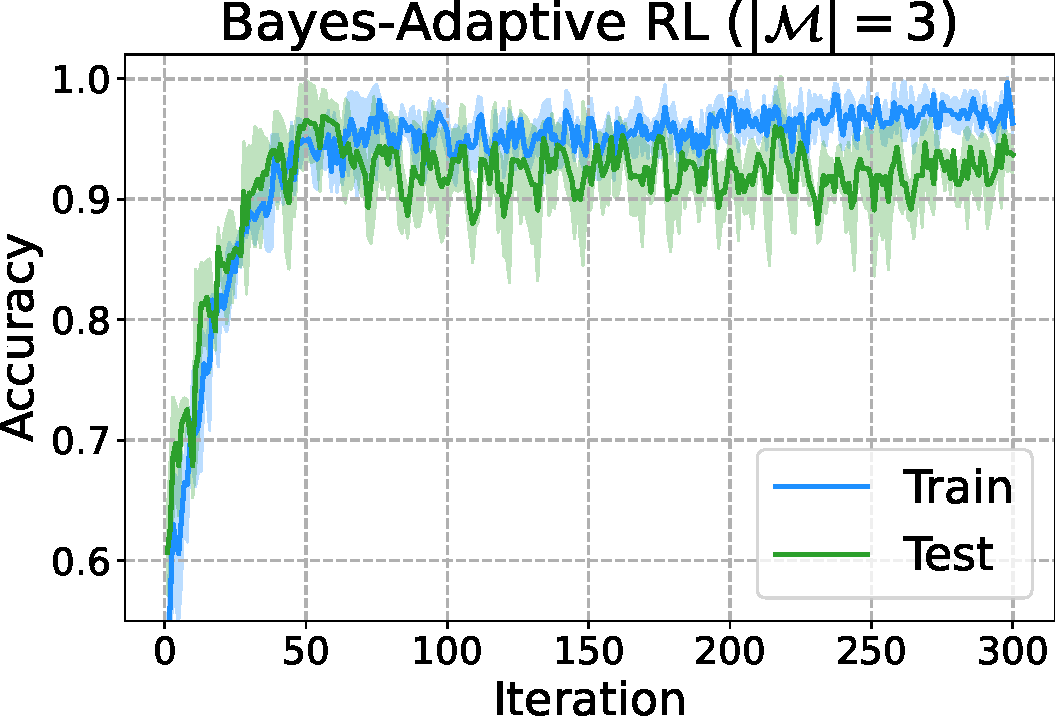
\includegraphics[width=0.96\linewidth]{figs/barl_reduced_example.pdf}
    \end{minipage}
\caption{Conventional RL (REINFORCE) memories training solutions and poorly generalizes beyond the training prompts. BARL performs well when deployed to the evaluation tasks and improves with more informative candidate sets.}
\label{fig_example_results}
\end{figure}